\documentclass[11pt]{article}

\usepackage{indentfirst}

\usepackage{graphicx}
\graphicspath{ {images/} }
\usepackage[rightcaption]{sidecap}
\usepackage{wrapfig}

\begin{document}

\title{Relat\'orio do Projeto Final de Programa\c{c}\~ao}
\date{Janeiro de 2018}
\author{In\^es Ferreira e Beatriz Marques}
\maketitle

\section*{Introdu\c{c}\~ao}

{
O presente relat\'orio refere-se ao desenvolvimento de um programa que simule um sistema constitu\'{i}do por duas molas (constante k), uma massa (massa M) e um p\^endulo (comprimento l e massa m) como representado Figura 1. O resultado 
final \'e apresentado na Figura 2.
}

\begin{figure}[ht]
    \centering
    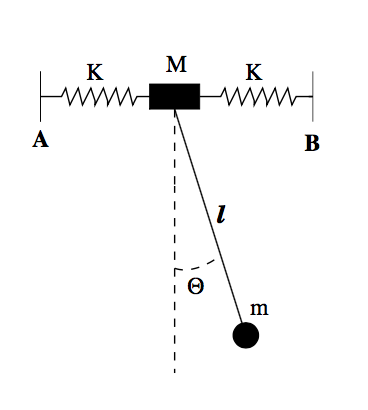
\includegraphics[width=0.25\textwidth]{figure3}
    \caption{Sistema op\c{c}\~ao 3}
\end{figure}

\begin{figure}[ht] \label{fig2}
    \centering
    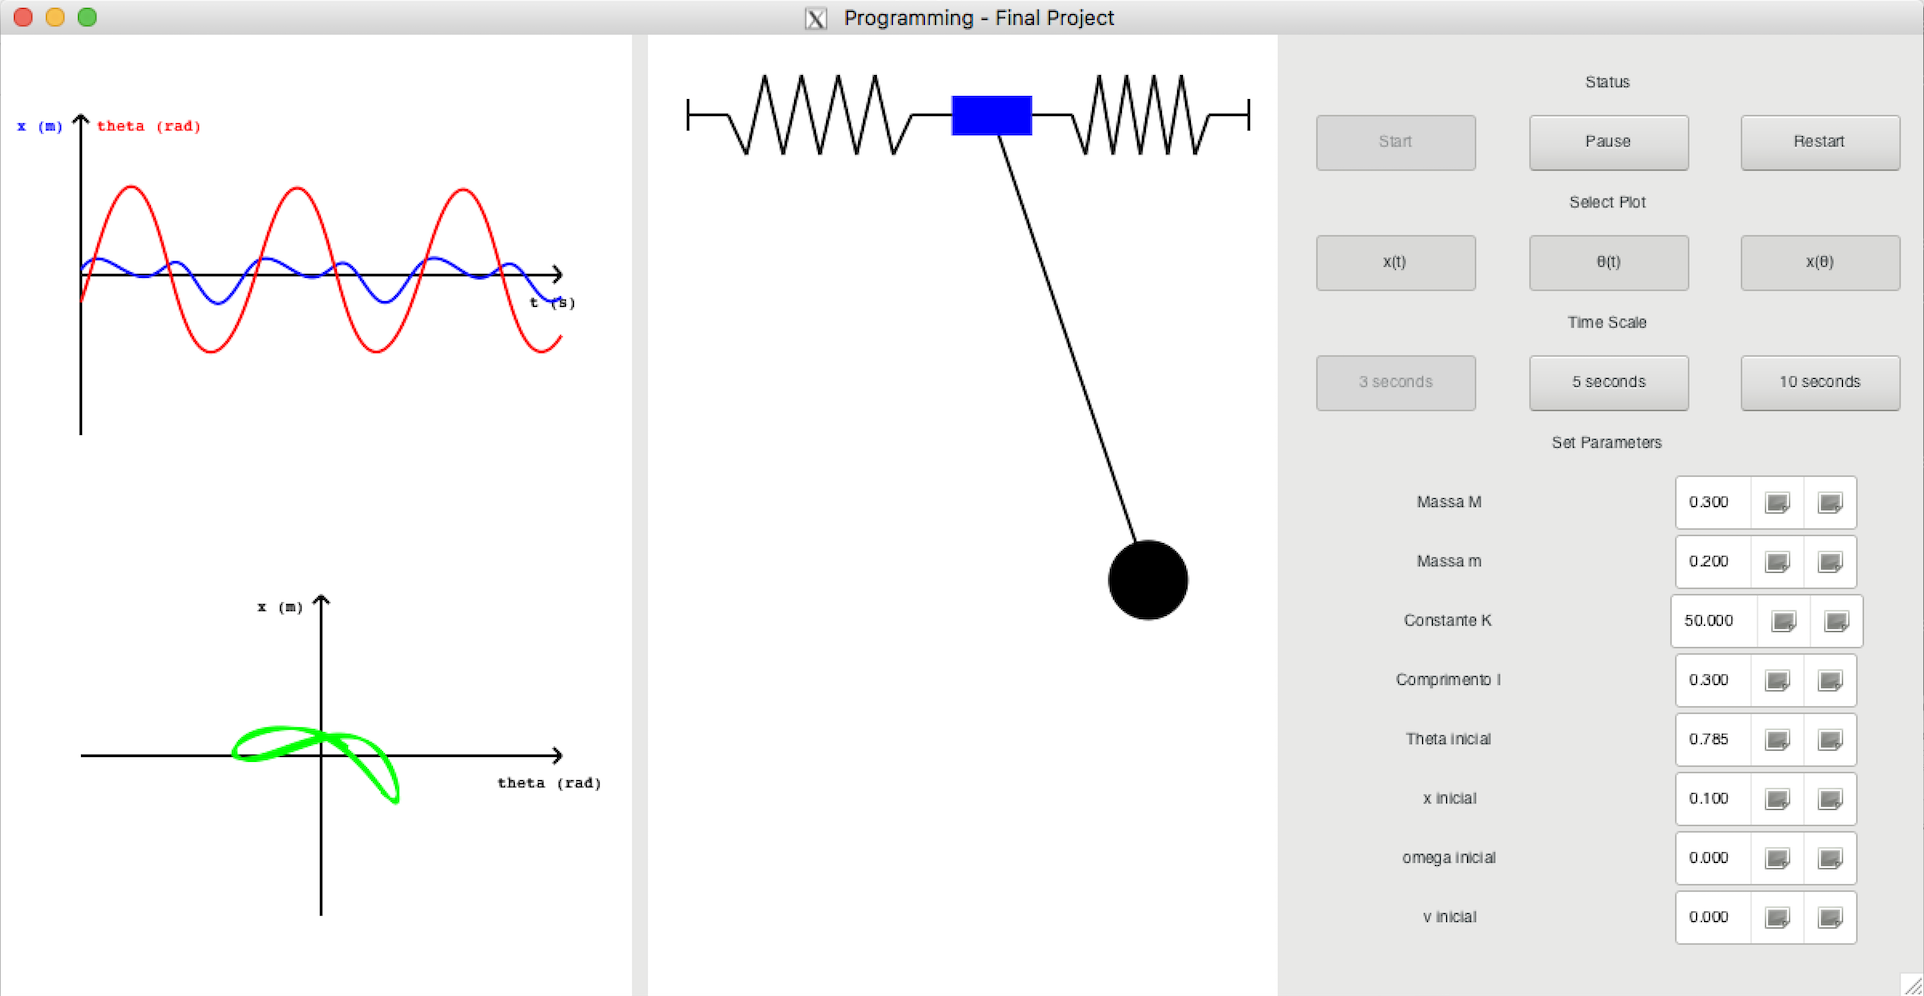
\includegraphics[width=1\textwidth]{figureprogram}
    \caption{Representa\c{c}\~ao Gr\'afica, Representa\c{c}\~ao Visual e Painel de Controlos }
\end{figure}

\section{Ficheiros auxiliares \textit{"data.c"} e \textit{"data.h"}}

{
O ficheiro \textit{"data.h"} tem as estruturas relativas \`{a} resolu\c{c}\~ao num\'erica das equa\c{c}\~oes. A estrutura \textit{"Consts"} cont\'em os valores atuais dos SpinButtons massa M, massa m, comprimento l e contante k. As estrutura \textit{"Coords"} cont\'em os valores de $\theta$, $x$, $v$ e $\omega$ necess\'arios a para a resolu\c{c}\~ao num\'erica.
\\
\indent
O ficheiro auxiliar "data.c" cont\'em as fun\c{c}\~oes (\textit{"newCoords"} e "newConsts") que geram as coordenadas e que alteram os valores das estruturas referidas anteriormente. A fun\c{c}\~ao "solver" resolve numericamente as equa\c{c}\~oes pelo m\'etodo de Euler-Cromer.
}

\section{Ficheiros auxiliares \textit{"circularbuffer.h"} e \textit{"circularBuffer.c"}}

{
O ficheiro \textit{"circularBuffer.c"} cont\'em diversas fun\c{c}\~oes que manipulam um vetor circular que servir\'a para guardar os valores das coordenadas $x$ e $\theta$ para cria\c{c}\~ao das representa\c{c}\~oes visual e gr\'afica. Este vetor ter\'a o tamanho m\'aximo de 1000 pontos para poder representar a maior escala de tempo (10 segundos).
}

\section{Ficheiro \textit{"main.c"}}

{
O \textit{"main.c"} come\c{c}a com a declara\c{c}\~ao das diversas estruturas. A estrutura \textit{"Widgets"} \'e relativa a componentes do \textit{Gtk}. A estrutura \textit{"data"} cont\'em um vetor circular para cada uma das coordenadas ($x$, $\theta$ e $t$), as coordenadas iniciais e as constantes. A estrutura \textit{"Global"}, para al\'em de conter as duas estruturas anteriores, tamb\'em tem presente duas vari\'aveis \textit{"status"} e \textit{"scale}" que representam o estado do sistema (\textit{"Start"} ou \textit{"Pause"}) e a escala de tempo dos gr\'aficos (3, 5 ou 10 segundos).
\\
\indent
A fun\c{c}\~ao "draw\_figure" desenha a figura com base nas coordenadas que est\~ao guardadas no vetor circular.
\\
\indent
A fun\c{c}\~ao \textit{"draw\_plot\_axis"} apenas desenha dois sistemas de eixos para os gr\'aficos. Na parte de cima da representa\c{c}\~ao gr\'afica s\~ao desenhados os gr\'aficos $\Theta(t)$ e $x(t)$, enquanto que em baixo fica apenas o gr\'afico  $x(\Theta)$. 
\\
\indent
A fun\c{c}\~ao \textit{"draw\_plot\_labels"} desenha as legenda dos eixos xx e yy em ambos os sistemas de gr\'aficos.
\\
\indent
A fun\c{c}\~ao \textit{"draw\_plot"} desenha cada um dos gr\'aficos lendo os valores do vetor circular e utilizando a escala escolhida pelo utilizador.
\\
\indent
A fun\c{c}\~ao \textit{"drawplotHandler"} chama sempre as fun\c{c}\~oes \textit{"draw\_plot\_axis"} e \textit{"draw\_plot\_labels"} para que os eixos apare\c{c}am sempre na figura mas apenas chama a fun\c{c}\~ao "draw\_plot" se o utilizador tiver ativado um ou mais dos bot~oes \textit{plot1}, \textit{plot2} e \textit{plot3}.
\\
\indent
A fun\c{c}\~ao \textit{"drawfigureHandler"} \'e semelhante \`{a} anterior, chamando a fun\c{c}\~ao \textit{"draw\_figure"}. A figura aparece sempre no ecr\~a, mas apenas se move se o \textit{"status"} igual a \textit{PLAY}.
\\
\indent
As fun\c{c}\~oes do tipo \textit{spinConstsHandler} permitem a atualiza\c{c}\~ao do valor das constantes e das coordenadas iniciais sempre que o valor dos \textit{SpinButtons} \'e alterado, ou seja, sempre que \'e emitido um sinal do tipo \textit{"value-changed"}.
\\
\indent
A fun\c{c}\~ao \textit{"timeHandler"} controla, de acordo com o \textit{"status"} do sistema, os contadores do tempo \textit{timer} e \textit{discrete\_timer}. Ou seja, as equa\c{c}\~oes apenas s\~ao resolvidas pela fun\c{c}\~ao \textit{"solver"} e os vetores circulares preenchidos se o bot\~ao \textit{"Start"} estiver ativado. 
\\
\indent
As fun\c{c}\~oes \textit{"buttonStartHandler"} e \textit{"buttonPauseHandler"} controlam a atividade e sensitividade dos but\~oes \textit{"Start"} e \textit{"Pause"}, ou seja, quando um deles est\'a ativo, o outro est\'a inativo. S\~ao estes bot\~oes que controlam o \textit{"status"} do sistema. A fun\c{c}\~ao \textit{"buttonRestartHandler"} coloca os contadores do tempo a zero e limpa os vetores circulares para que o gr\'afico tamb\'em se "apague" quando o bot\~ao \textit{"Restart"} \'e presionado.
\\
\indent
As fun\c{c}\~oes \textit{"buttonScale1Handler"}, \textit{"buttonScale2Handler"} e \textit{"buttonScale3Handler"} permitem fazer a escolha da escala do tempo do gr\'afico, alterando a vari\'avel global \textit{"scale"}.

O main do ficheiro come\c{c}a com a inicializa\c{c}\~ao das vari\'aveis criando os vetores circulares e com a implementa\c{c}\~ao das coordenadas inciais e cont\'em todos os dados relativos aos \textit{Widgets} do \textit{Gtk}.
}

\end{document}
